\section{Comparison between networks}
Lastly it is possible to see how each architecture compares with one another in the experiments made. This was done here by taking the three best results for each architecture in each dataset and highlighting their metrics accordingly. \autoref{fig:comparison_architectures} shows the resulting comparison.
\begin{figure}[hbt]
    \caption{Comparison of different GAN architectures performances}
    \centering
        \begin{subfigure}[b]{\textwidth}
        \centering
        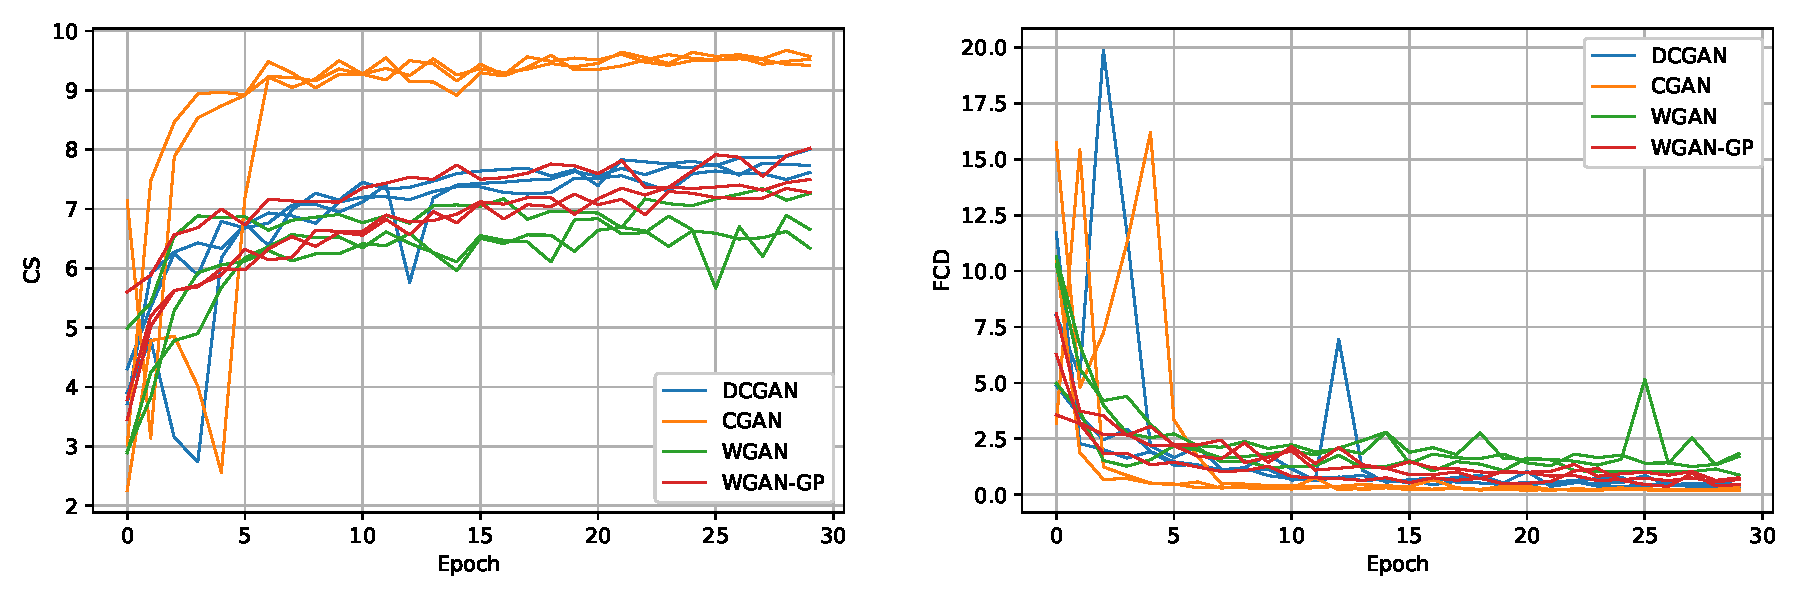
\includegraphics[width=\textwidth]{chapters/Experiments/Comparison/Comparison_MNIST.pdf}
        \caption{MNIST}
        \end{subfigure}
        
        \begin{subfigure}[b]{\textwidth}
        \centering
        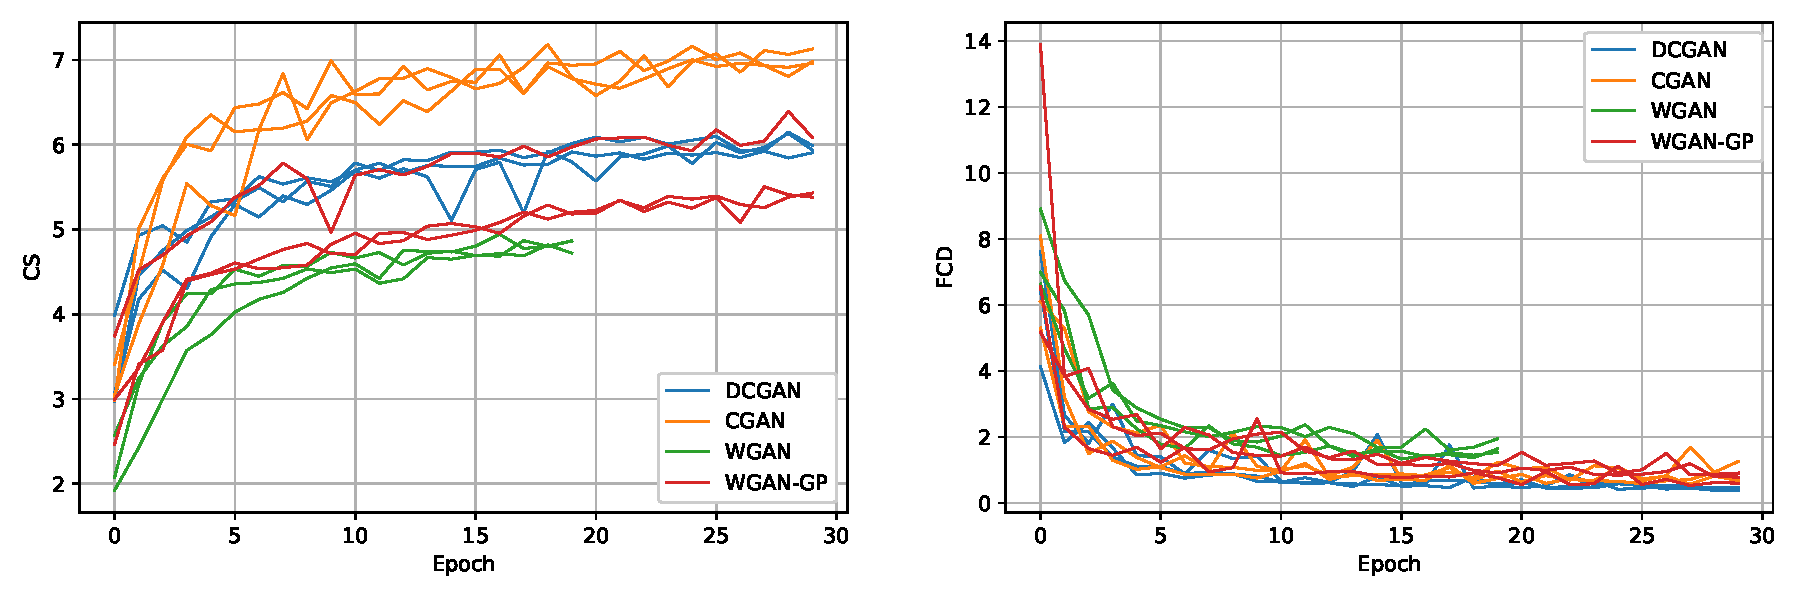
\includegraphics[width=\textwidth]{chapters/Experiments/Comparison/Comparison_Fashion.pdf}
        \caption{Fashion MNIST}
        \end{subfigure}
        
        \begin{subfigure}[b]{\textwidth}
        \centering
        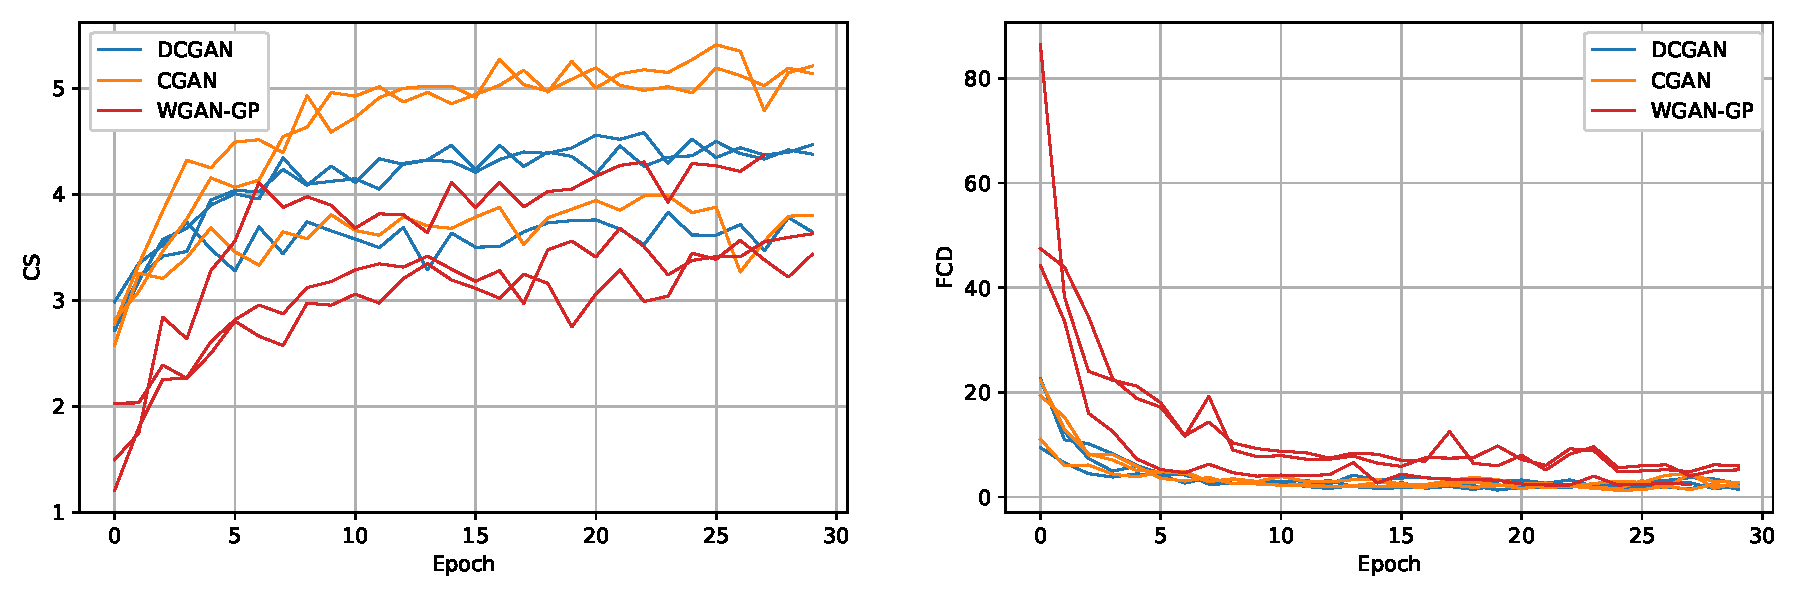
\includegraphics[width=\textwidth]{chapters/Experiments/Comparison/Comparison_CIFAR.pdf}
        \caption{CIFAR-10}
        \end{subfigure}
    \fonte{From the author (2021)}
    \label{fig:comparison_architectures}
\end{figure}

The best model shown here by far is clearly the \gls{CGAN}, however, as \textcite{nipsGAN2017} puts it, this is an unfair comparison. It is important to note that this model has extra information in which to base it's output, the quality of the results do not come from a cleverly built network, but by the data itself. This is not a useful way of evaluating the architecture on it's own.

It is also important to mention that the \gls{CGAN} implemented for this document is just a \gls{DCGAN} with label conditioning, the same could be made for the \gls{WGAN} and \gls{WGAN-GP}. \autoref{fig:comparison_architectures} includes the \gls{CGAN} only to give an idea of how much labels can help, but the important comparisons are between the other three models.

From the remaining models the \gls{WGAN} showed the weakest results, this may not necessarily be the case for all tests, since \textcite{wasserstein2017} showed good results in the high resolution LSUN Bedrooms dataset with this architecture. More tests would be ideal in order to make more definitive statements, but the results seen in these experiments weren't able to reproduce performances similar to the ones for \gls{DCGAN} or \gls{WGAN-GP}, and they also showed a moderate level of instability in the choice of hyperparameters.

The problem of \gls{WGAN} is mostly due to the implementation of weight clipping, the \gls{WGAN-GP} offers a better way of maintaining the Lipschitz continuity without losing the good properties of the Wasserstein loss. It showed similar results to the \gls{DCGAN} for all datasets, but it has the added benefit of being more stable, the hyperparameter search did not need to be so expansive.
